\documentclass{jlreq}

\usepackage{graphicx}
\usepackage[hidelinks]{hyperref}
\usepackage{listings}
\usepackage{amsmath}

\begin{document}
    \begin{titlepage}
        \centering
        {\large システム提案書  第1.0版\par}
        \vspace{2cm}

        {\LARGE \textbf{アプリの名前}\par}
        \vspace{2cm}

        {\large YHY\par Group 12\par}
        \vspace{2cm}
        {\large \today \par}
    \end{titlepage}

    % 現状の課題
    % \section{現状の課題}
\subsection{アンケート結果による現状の分析}
土佐山田町の地域情報の入手状況と地域SNSに必要な情報及び機能についてアンケートを実施した.アンケートは土佐山田町に住む10代から50代の男女30名に実施した.

\subsubsection{地域のイベントやお店の情報をどのくらいチェックしていますか?}
\begin{figure}[H]
    \centering
    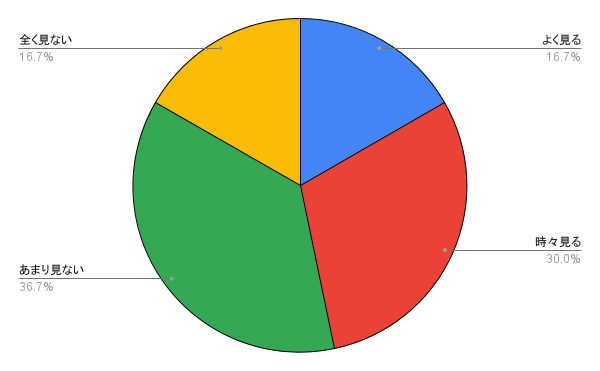
\includegraphics[width=0.5\linewidth]{fig125/Q1.png}
    \caption{地域情報等を見る頻度}
    \label{fig:Q1}
\end{figure}
図\ref{fig:Q1}より,5割程度の人が土佐山田町に関する情報をあまり見ない,全く見ないと回答している.

\subsubsection{地域情報は普段どこから得ていますか?(複数回答可)}
\begin{figure}[H]
    \centering
    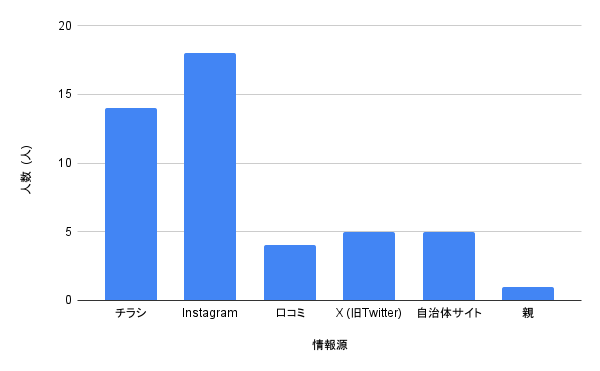
\includegraphics[width=0.5\linewidth]{fig125/Q3.png}
    \caption{地域情報の入手先}
    \label{fig:Q3}
\end{figure}
図\ref{fig:Q3}より,地域情報は主にInstagram (約36\%) やチラシ (約32\%)から得ていることが分かった.

\subsubsection{どんな情報を地域SNSで見たいですか?(複数回答可)}
\begin{figure}[H]
    \centering
    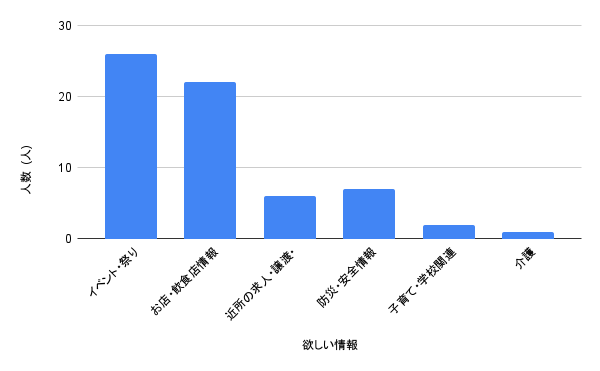
\includegraphics[width=0.5\linewidth]{fig125/Q4.png}
    \caption{見たい地域情報}
    \label{fig:Q4}
\end{figure}
図\ref{fig:Q4}より,地域SNSがあるならば,イベント情報 (40\%) や飲食店の情報 (約33\%)を入手したい人が多いことが分かった.

\subsubsection{どんな機能があれば使いたいと思いますか?}
\begin{figure}[H]
    \centering
    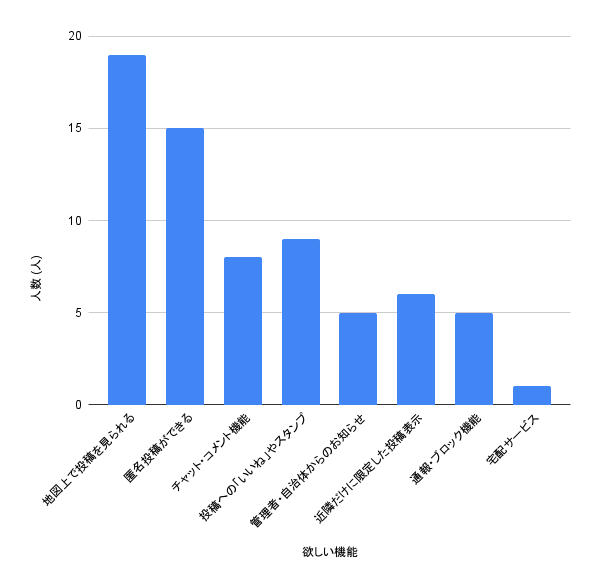
\includegraphics[width=0.5\linewidth]{fig125/Q7.png}
    \caption{欲しい機能}
    \label{fig:Q7}
\end{figure}
図\ref{fig:Q7}より,地域SNSに欲しい機能として地図上での投稿の閲覧 (約29\%),匿名投稿 (約23\%)を上げる人が多かった.

\subsection{アンケート結果の分析}
アンケートの結果より土佐山田町に住んでいる人は地域情報を積極的に入手する人は少ないことが分かる.これは,土佐山田町の地域情報を発信している媒体が複数存在しており,情報が分散されていることが原因と考えられる.例として,香美市の公式サイト\cite{label1}では以下の以下の5つの項目を確認できる.
\begin{enumerate}
    \renewcommand{\labelenumi}{・}
    \item くらしの情報
    \item 事業者向け情報
    \item 観光・イベント情報
    \item 市政情報
    \item 施設検索
\end{enumerate}
住民生活に関係するくらしの情報の項目では福祉,税金,交通情報,防災・災害などの18項目を取り扱っている.香美市では以下の6つを公式SNSとして運用している\cite{label2}.
\begin{enumerate}
    \renewcommand{\labelenumi}{・}
    \item 香美市公式LINE
    \item 香美市公式Facebook
    \item 香美市立図書館公式Instagram
    \item 香美市あんぱん室(やなせたかし先生顕彰事業推進室)公式Instagram
    \item 香美市消防本部公式Instagram
    \item 香美市山村留学公式Instagram
\end{enumerate}
公式LINEではイベントの情報を中心に,公式Facebookでは活動報告を中心に発信している.
Instagramは4つ公式アカウントがあるように分野別にアカウントを分けて発信している.これらの公式SNSに加えて,土佐山田町にある企業や店舗の発信や個人的な発信が様々な媒体で行われている.そのため,必要な情報を得るために複数の媒体を利用しなければならない現状がある.

しかし,アンケート結果の図\ref{fig:Q4}より,地域のイベントの情報や飲食店の情報を求めている人が多く,これらの情報はアンケート結果の図\ref{fig:Q7}で多くの人が欲しい機能として挙げた地図上で投稿が見られるようにするという機能との相性が良いと考えられる.

    % 課題解決のための提案
    % \section{課題解決のための提案}
土佐山田町の地域情報を積極的に入手していないこととイベントや飲食店の情報を入手できるようにするために土佐山田町の情報に特化したSNSを提案する.このSNSにより自治体や,企業,個人の発信をまとめることで情報の集約化を行い,情報収集の効率を上げる.また,このSNSが普及することで地域活性化が期待できる.

\subsection{情報の集約化}
アンケートの結果図\ref{fig:Q1}より,土佐山田町に住んでいる人は地域の情報を積極的に入手している人が少ない.これは,土佐山田町の情報を発信している媒体が複数あり,情報を収集する意欲が起きにくいことが原因であると考えられる.そこで,土佐山田町の情報に特化したSNSを作成することで情報を集約化し,情報収集にかける時間と労力を減らすことが期待できる.

\subsection{情報収集の効率化}
総務省の情報通信白書のSNSの項目より,日本のソーシャルメディアの利用者は1億580万人となっており,今後も緩やかに増加していくと見られている.使用されているメディアとしてはFacebook,Instagram,X(旧Twitter)が主流である,このことから,主流のソーシャルメディアに1日あたりに投稿される数は膨大であることが予想できる.そのため,情報収集をするには膨大な情報の中から必要な情報を見つけ出さなければならず,効率的でないと言える.そこで,土佐山田町の情報に特化したSNSを作成することで,メディアに存在する情報量を少なくして,情報収集の効率を上げることができると予想できる.

\subsection{地域活性化}
アンケートの結果図\ref{fig:Q4}より,イベント情報や飲食店の情報を知りたいという回答が多かった.また,図\ref{fig:Q7}より,地図上での投稿の閲覧機能を挙げた人が多かった.このことから,地図上にイベント情報や飲食店の情報をできるようにすることで多くの利用者を見込めることになると考える.また,このSNSに投稿されたイベントの情報や飲食店の情報を見た利用者が,実際にイベントへの参加や飲食店への来店をすることで地域活性化が期待できる.

    % 機能概要・前提条件・制約事項
    % \section{機能概要・前提条件・制約事項}
\subsection{機能概要}
\subsubsection{一般向け}
\begin{itemize}[itemsep=10pt]
    \item 会員機能
    \begin{itemize}[itemsep=10pt]
        \item 新規会員登録 \mbox{}\\
        一般会員がGoogleアカウントを用いて会員になる機能.また,新規会員登録の際に利用規約を提示し,規約に従う場合にのみ新規登録を行う.
        \item ログイン・ログアウト \mbox{}\\
        ログイン機能では一般会員がGoogleアカウントを用いた認証機能により認証を行うことで本システムにログインをする.ログアウト機能では本システムにすでにログインしている会員が任意のタイミングでログアウトすることができる.
        \item 退会 \mbox{}\\
        退会機能では会員が任意のタイミングで本システムから退会することのできる機能.退会した会員の情報は退会処理が終了した時点で完全に消去する.
        \item 問い合わせ \mbox{}\\
        一般会員が質問や要望を運営側に問い合わせることができる機能.質問や要望はメール形式で送信され,運営側からの回答は本システム会員が登録しているGoogleアカウントのメールアドレスへ送信される.
        \item 事業者登録申請機能 \mbox{}\\
        一般会員から事業者会員への昇格を運営側へ申請する機能.店舗名,電話番号,店舗の住所などの情報を入力し運営からの承認を経て事業者会員となる.
    \end{itemize}
    \item ピン表示機能
    \begin{itemize}[itemsep=10pt]
        \item 地図上でのピン表示 \mbox{}\\
        他の会員が投稿したピンを地図上に視覚的に表示する機能.この際,一般会員が投稿したピンは円で表示される.同一地点に存在するピンの数に応じて表示されるピンの大きさが段階的に変化する.
        \item ジャンル分け機能 \mbox{}\\
        投稿の内容に応じてジャンルを選択できる機能.ジャンルに応じてピンの色が変化する.
        \item  リアクション機能 \mbox{}\\
        各ピンに対してほかの一般会員からのリアクションを表示する機能.このリアクションは匿名でのリアクションであり,リアクションの数のみが表示される.
    \end{itemize}
    \item 絞り込み機能
    \begin{itemize}[itemsep=10pt]
        \item キーワード \mbox{} \\
        検索窓を利用して,入力したキーワードに応じて情報を検索・絞り込みできる機能.
        \item ジャンル \mbox{}\\
        特定のジャンルに属するピンのみを表示する機能.
        \item 日にち \mbox{}\\
        指定した日付または期間内に投稿されたピンのみを表示する機能.
    \end{itemize}
    \item 並べ替え機能
    \begin{itemize}[itemsep=10pt]
        \item 距離順 \mbox{} \\
        現在地または任意の場所からの距離が近い順にピンの表示を並べ替える機能.
        \item リアクション数順
        リアクションの数が多い順または少ない順にピンの表示を並べ替える機能.
    \end{itemize}
    \item ピン投稿機能
    \begin{itemize}[itemsep=10pt]
        \item 場所情報投稿機能 \mbox{}\\
        一般会員自身が匿名で任意の場所を地図上にピンとして投稿できる機能.投稿時は位置情報を地図上で指定または事業者名で検索により入力.
        \item 記述・写真情報投稿機能 \mbox{}\\
        一般会員自身がつけたピンに対して説明文等のテキスト,写真情報を投稿できる機能.
        \item 時間情報登録機能 \mbox{}\\
        ピンの投稿,記述・写真を投稿した際の時刻を登録する機能.
        \item ジャンル登録機能 \mbox{}\\
        投稿内容のジャンルを登録できる機能.
    \end{itemize}
    \item マイページ
    \begin{itemize}[itemsep=10pt]
        \item リアクション履歴閲覧機能 \mbox{}\\
        一般会員自身がこれまでにリアクションを行った投稿の履歴を閲覧できる機能.
        \item 投稿履歴閲覧機能 \mbox{}\\
        一般会員自身がこれまでに投稿したピン投稿の履歴を一覧で確認できる機能.
        \item 投稿内容削除機能 \mbox{}\\
        一般会員自身がこれまでに投稿したものを削除できる機能.
    \end{itemize}
    \item 通報機能 \mbox{} \\
    一般会員が不適切な投稿に対して管理者へ報告を行うことができる機能.
    \item ブロック機能 \mbox{} \\
    一般会員が特定のユーザに対してブロックすることができる機能.ブロックを行うと相手の投稿や相手からのリアクションが表示されなくなる.
\end{itemize}

\subsubsection{事業者向け}
\begin{itemize}[itemsep=10pt]
    \item 会員機能
    \begin{itemize}[itemsep=10pt]
        \item ログイン・ログアウト \mbox{}\\
        ログイン機能では事業者会員がGoogleアカウントを用いた認証機能により認証を行うことで本システムにログインをする.ログアウト機能では本システムにすでにログインしている会員が任意のタイミングでログアウトすることができる.
        \item 退会 \mbox{}\\
        退会機能では会員が任意のタイミングで本システムから退会することのできる機能.退会した会員の情報は退会処理が終了した時点で完全に消去する.
        \item 問い合わせ \mbox{}\\
        事業者会員が質問や要望を運営側に問い合わせることができる機能.質問や要望はメール形式で送信され,運営側からの回答は本システム利用者が登録しているGoogleアカウントのメールアドレスへ送信される.
    \end{itemize}
    \item ピン表示機能
    \begin{itemize}[itemsep=10pt]
        \item 地図上でのピン表示 \mbox{}\\
        他の会員が投稿したピンを地図上に視覚的に表示する機能.事業者会員が投稿したピンはピンの真ん中にロゴが表示される.同一地点に存在するピンの数に応じて表示されるピンの大きさが段階的に変化する.
        \item ジャンル分け機能 \mbox{}\\
        投稿の内容に応じてジャンルを選択できる機能.ジャンルに応じてピンの色が変化する.
    \end{itemize}
    \item ピン投稿機能
    \begin{itemize}[itemsep=10pt]
        \item 場所情報投稿機能 \mbox{}\\
        事業者会員自身が任意の場所を地図上にピンとして投稿できる機能.投稿時は位置情報を地図上で指定また事業者名で検索により入力.事業者会員が投稿した場合は事業者名または店舗名がピンに表示される.
        \item 記述・写真情報投稿機能 \mbox{}\\
        事業者会員自身がつけたピンに対して説明文等のテキスト,写真情報を投稿できる機能.
        \item 時間情報登録機能 \mbox{}\\
        ピンの投稿,記述・写真を投稿した際の時刻を投稿する機能.
        \item ジャンル登録機能 \mbox{}\\
        投稿内容のジャンルを登録できる機能.
    \end{itemize}
    \item マイページ
    \begin{itemize}[itemsep=10pt]
        \item 投稿履歴閲覧機能 \mbox{}\\
        事業者会員自身がこれまでに投稿したピン投稿の履歴を一覧で確認できる機能.
        \item 投稿内容削除機能 \mbox{}\\
        事業者会員自身がこれまでに投稿したものを削除できる機能.
        \item ダッシュボード機能 \mbox{} \\
        事業者会員自身がこれまでに投稿に対するリアクション数の推移や閲覧数を閲覧できる機能.
        \item 支払い状況確認機能 \mbox{} \\
        現在の契約状況や支払い履歴,次回の請求日・支払額が確認できる機能.事業者会員からの解約もこのページから行うことができる.
    \end{itemize}
\end{itemize}

\subsubsection{管理者}
\begin{itemize}[itemsep=10pt]
    \item 投稿の削除機能 \mbox{}\\
    管理者が不適切な投稿や規約に違反する投稿を削除できる機能.削除後はシステム上から該当投稿を完全に削除し,該当するアカウントに通知する.
    \item アカウントの削除機能 \mbox{}\\
    管理者が利用規約違反や不正行為を行ったアカウントを凍結できる機能.削除に伴い,関連する投稿・リアクション情報も一括で消去される.
    \item 事業者アカウントへの変更 \mbox{}\\
    管理者が申請のあった一般会員アカウントを事業者会員アカウントへ変更できる機能.事業者認証および事業者側からの支払い方法の登録確認後,事業者向けの機能が利用可能となる.
    \item 問い合わせへの対応機能 \mbox{} \\
    一般会員,事業者会員からの問い合わせに対して答える機能.
    \item 運用状況モニタリング機能 \mbox{} \\
    これまでのアクティブユーザー数や新規投稿の推移,最も人気の高い投稿やサーバーの負荷状況を確認することができる機能.
\end{itemize}

\subsection{前提条件}
本提案書では以下の条件を前提条件とする.
\begin{itemize}
    \item 利用者がインターネットに接続可能な端末 (スマートフォンや PC など) を保有していること.
    \item 利用者が本システムの規約に同意済みであること.
    \item 利用者がGoogleアカウントを所有していること.
    \item 1Googleアカウントに対して本システムの1アカウントの所持のみとすること.
\end{itemize}

\subsection{制約事項}
本システムの制約事項を以下に示す.
\begin{itemize}
    \item 利用者の個人情報漏洩を防ぎ,保護する仕様であること.
    \item 利用者の個人情報を編集できない仕様であること.
    \item 管理者側による投稿の削除・規制が行える仕様であること.
\end{itemize}

    % 情報・金銭の流れ
    % \section{情報・金銭の流れ}
\subsection{情報の流れ}
本システムは,管理者端末,利用者端末の2つの端末と Amazon WebServise(AWS) 内の WEB/AP サーバ,データベースおよびストレージとそれを繋ぐインターネットによって構成されている.図 \ref{fig:Q7}に各端末とサーバが通信する情報の流れを示す.管理者,利用者は,必要な情報を AWS 内のデータベースなどに要求することで,情報の提供が行われ,要求に応じた各システムの処理が行われる.

\begin{figure}[H]
        \centering
        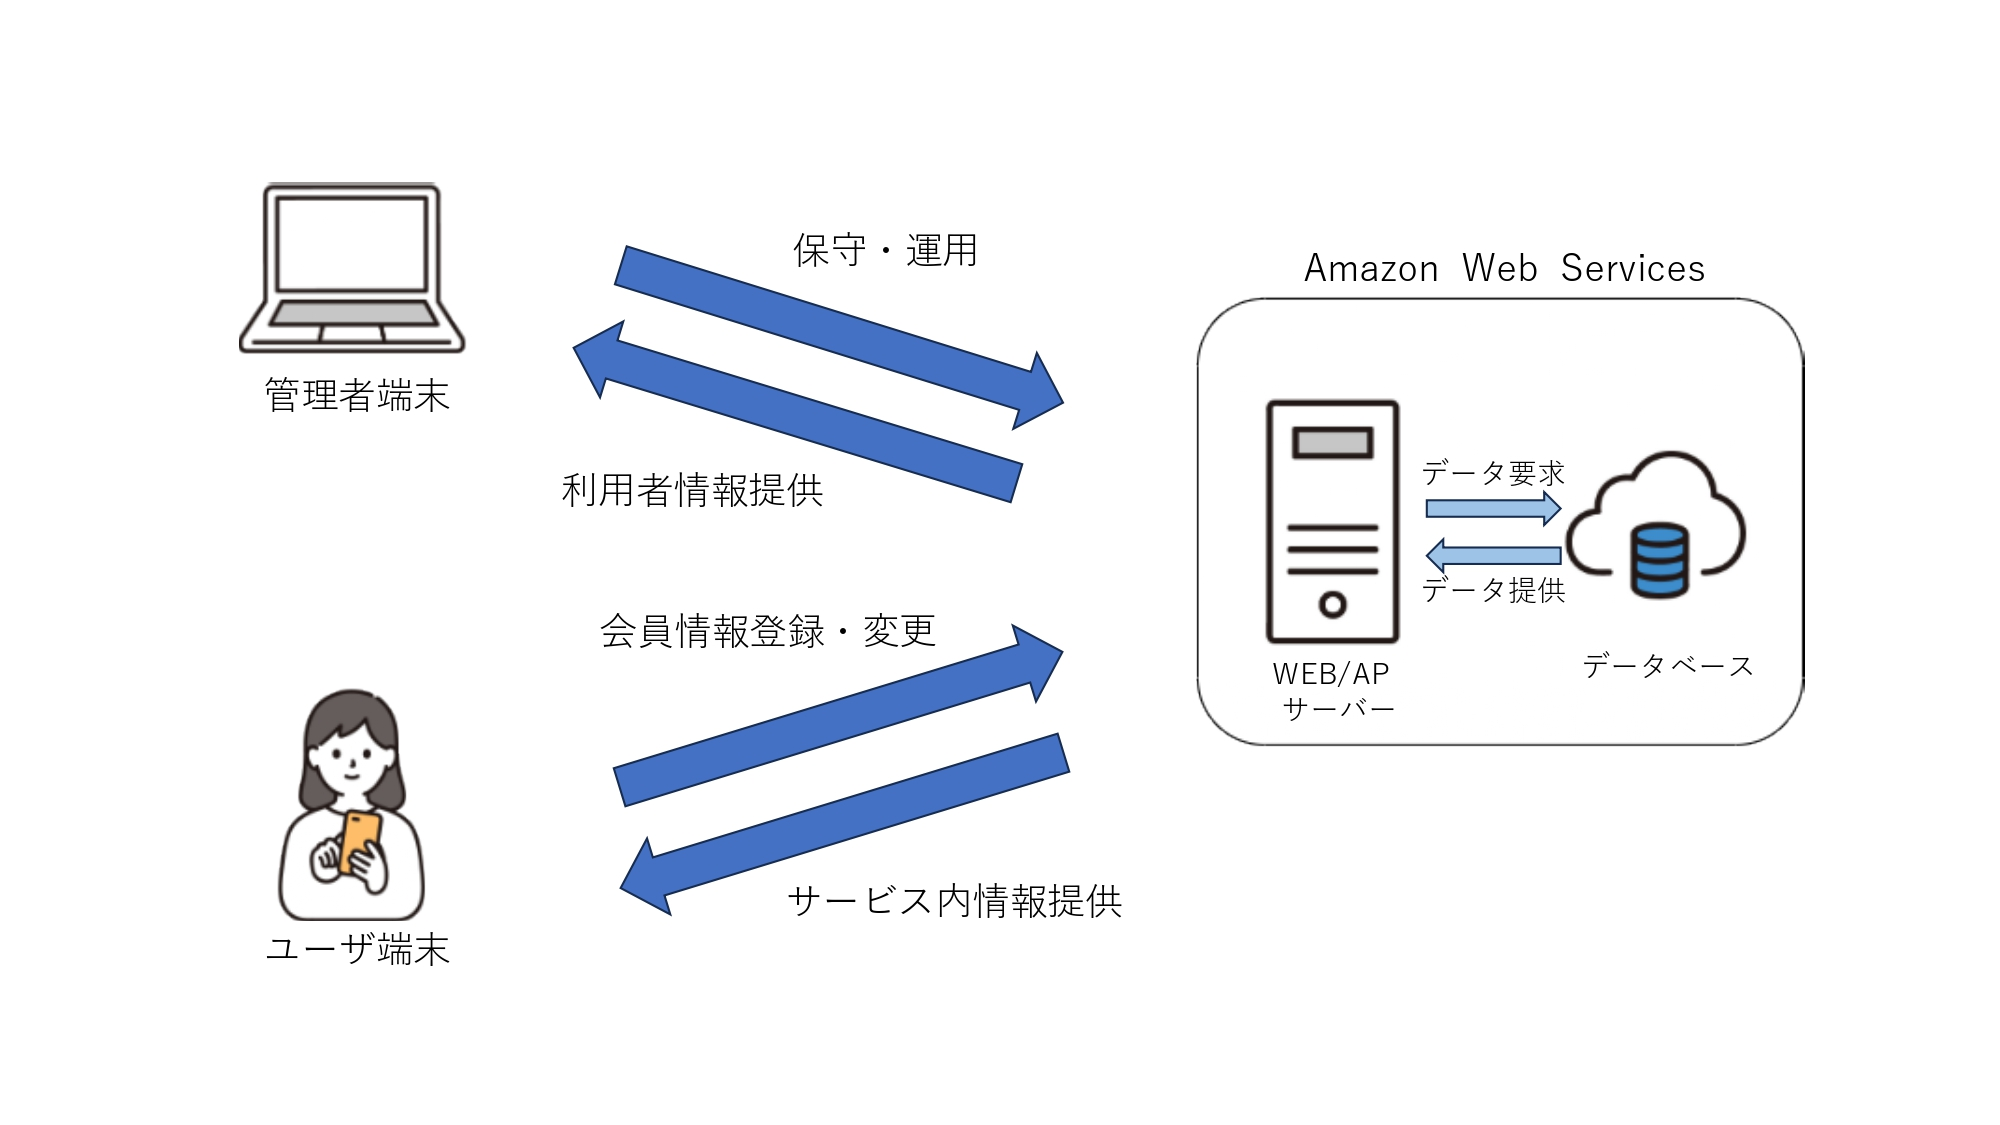
\includegraphics[width=12cm, height=7cm]{pictures/4-1_info.jpg}
        \caption{情報の流れ}
        \label{fig:Q7}
\end{figure}



\subsection{金銭の流れ}
金銭の流れは,図\ref{fig:Q8}に示す.

\begin{figure}[H]
        \centering
        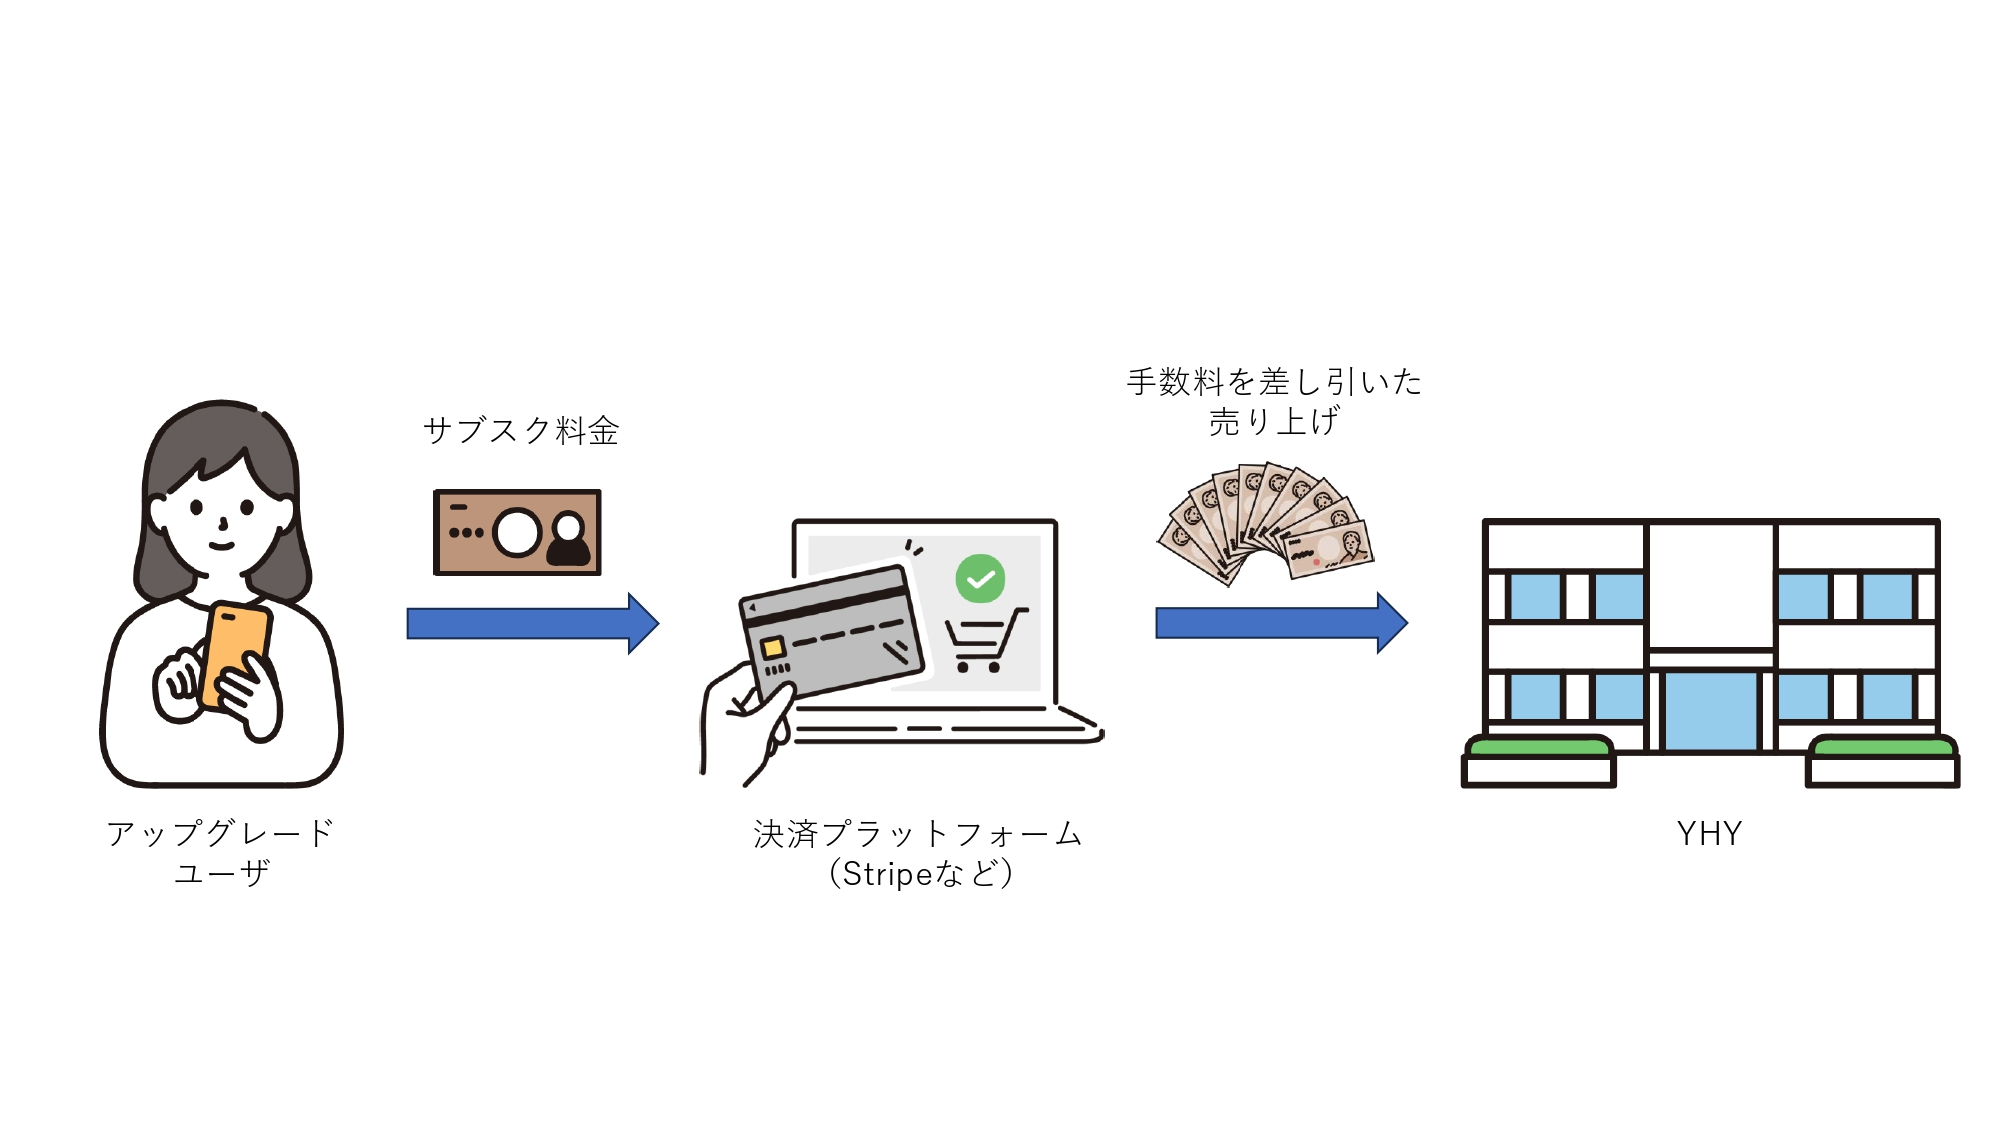
\includegraphics[width=12cm, height=7cm]{pictures/4-2_money.jpg}
        \caption{金銭の流れ}
        \label{fig:Q8}
\end{figure}

事業者会員は,クレジットカードなどを用いてサブスクリプション料金を支払う.この支払いは直接弊社に送金されるのではなく,決済プラットフォームを経由して処理される仕組みである。決済プラットフォームは,利用者から受け取った料金から決済手数料(数%程度)を差し引いたうえで、残額を弊社に振り込む.この入金は即時ではなく,一定期間(例:1 週間または 1 か月)分をまとめて支払われる.そのため,弊社が実際に受け取る金額は,利用者の支払総額から手数料を差し引いた純売上となる.









    % 想定する利用者
    % \section{想定する利用者}
想定される利用者は以下の通りである.
\begin{enumerate}
    \renewcommand{\labelenumi}{・}
    \item 土佐山田町に在住している人
    \item 土佐山田町の自治体職員
    \item 土佐山田町でお店を経営している人
\end{enumerate}


    % ハードウェア想定・ソフトウェア想定
    % \section{ハードウェア構成・ソフトウェア構成}
本システムの開発に用いるハードウェアおよびソフトウェアの構成を以下に示す.
\subsection{ハードウェア構成}
\begin{table}[]
    \centering
    \caption{ハードウェア構成}
    \label{tab:hardware}
    \begin{tabular}{llll}
    \hline
    項目         & 種類          & 数量   & 備考 \\ \hline
    メインサーバー    & レンタルサーバー    & 2    &    \\
    データベースサーバー & レンタルサーバー    & 2    &    \\
    管理者端末      & PC          & 1    &    \\
    利用者端末      & スマートフォンやPC等 & 利用者数 &    \\ \hline
    \end{tabular}
\end{table}

\subsection{ソフトウェア構成}
\begin{table}[]
    \centering
    \caption{ソフトウェア構成}
    \label{tab:software}
    \begin{tabular}{lll}
    \hline
    項目      & ソフトウェア                               & 備考 \\ \hline
    バックエンド  & GO                                   &    \\
    フロントエンド & TypeScript                           &    \\
    DB      & MySQL                                &    \\
    管理者端末   & Mac                  &    \\
    利用者端末   & Mac, Windows, Linux, iPhone, Android &    \\
    開発環境    & Docker                               &    \\
    クラウド    & AWS EC2                              &    \\
    CI/CD   & GitHub Actions                       &    \\
    認証基盤    & Google OAuth 2.0                     &    \\ \hline
    \end{tabular}
\end{table}

    % 運用・保守
    % \section{運用・保守}
システムの運用・保守に関しては以下の通りである.
\subsection{運用}
\begin{itemize}
    \item システム稼働状況や不具合がないかなどの監視
    \item データのバックアップ
    \item 外部からの攻撃や情報流出などの監視
    \item システム障害復帰からの再起動
    \item 問い合わせへの対応
\end{itemize}

\subsection{保守}
\begin{itemize}
    \item ネットーワークなどのインフラのメンテナンス
    \item バグや不具合の原因究明
    \item システムのアップデート
    \item 修正ログのバックアップ
\end{itemize}

    % 費用対効果
    % \section{費用対効果}
\subsection{効果}
本システムの導入により,地域住民が身近な出来事やイベント情報を地図上で共有できるようになる.ピン表示機能によって地域内の情報が視覚的に整理され,ジャンルごとの
色分けやリアクション機能を通じて,住民間の関心の傾向や交流の動向が可視化される.これにより,従来は口コミや限定的な SNS投稿に留まっていた地域の小規模な活動や話題
が広く共有され,地域内での情報循環が活発化する.\par
また,ジャンルや日付による絞り込み機能により,利用者は自分の興味関心や予定に合わせて地域イベントや活動を容易に発見できる.清掃活動,ボランティア,祭り,防災訓
練などへの参加が促進され,地域社会における住民参加率と情報発信率の向上が期待できる.さらに,投稿データの蓄積によって,地域ごとの関心分野や活動傾向を定量的に把握
できるため,自治体や地域団体が実証的データに基づく地域施策の立案・改善を行いやすくなる. \par
これらの仕組みにより,地域内の情報流通と住民参加が循環的に強化され,地域社会の協働性および自律的な活動基盤の形成が促進される.

\subsection{費用}
本システムの開発及び運用における費用をそれぞれ表\ref{fig:Q10},\ref{fig:Q11}に示す.
\clearpage

\begin{table}[h]
  \centering
  \caption{開発費}
  \label{fig:Q10}
  \begin{tabular}{crcrc}
  \hline
  項目  & 単価(円) & 数量   & 4ヶ月分換算費用(円) & 備考\\ \hline\hline
  
メインサーバ  & 約5,000円/月 & 2  & 約40,000円&  \\ \hline

データベースサーバ & 約4,000円/月 & 2  & 約32,000円& \\\hline

クラウド(AWS EC2) &約10,000円/月 &1 & 約40,000円& 小規模用を想定\\ \hline

管理者端末(PC) & 約120,000円/台& 1& 約120,000円& 5年間使用想定 \\ \hline

人件費  & 約400,000円/月 & 7& 約11,200,000円& 給料のみを想定\\ \hline\hline

合計 & & & 約11,432,000円\\ \hline
\end{tabular}
\end{table}



\begin{table}[h]
  \centering
  \caption{運用維持費}
  \label{fig:Q11}
  \begin{tabular}{crccr}
  \hline
  項目  & 単価(円) & 数量  & 期間 & 換算費用(円) \\ \hline\hline
 
メインサーバ  & 約5,000円/月 & 2& 60ヶ月  & 約600,000円 \\ \hline

データベースサーバ & 約4,000円/月 &2& 60ヶ月 & 約480,000円 \\\hline

クラウド(AWS EC2)  &約10,000円/月&1 &60ヶ月 & 約600,000円 \\ \hline\hline

合計 &  & & & 約1,680,000円\\ \hline
\end{tabular}
\end{table}

以上より,本システムを開発・5年間運用するために必要な費用は以下である.
\begin{table}[h]
  \centering
  \caption{費用総額}
  \label{fig:Q12}
  \begin{tabular}{ccc}
  \hline
  開発費 & 運用費 & 総額  \\ \hline\hline
 約11,432,000円 & 約1,680,000円 & 約13,112,000円\\ \hline

\end{tabular}
\end{table}


\subsection{収益・利益}
以下の式は,5年間で得られる収益を計算している.5年間でかかる費用は,表\ref{fig:Q12}より,12,572,000円である.\par
土佐山田町全体の事業者数は約1200店舗であり,そのうち広告対事業者は約435店舗である.約435店舗のうち,130店舗が本システムのサブスク機能を利用すると仮定する.

本システムは,企業用を使用する場合は5000円/月の利用料を設定する.この時,130店舗から月々5000円を徴収することで5年間の運用利益は以下になる.\par

\[5000(円)\times 60(ヶ月)\times 130(店舗)=39,000,000円(収益)\]


5年間で見込まれる収益から,5年間でかかる費用を差し引くと,本システムによって得られる5年間の利益は以下になる.

\[39,000,000円(収益)-13,112,000円(開発・運用費)=25,888,000円(利益)\]
これにより2年で開発・運用費を回収することができる.










    % 開発体制と工程計画
    % \section{開発体制と工程計画}
本システムは,弊社のメンバー7名によって開発を行う.\par
ウォーターフォールモデルを採用し,下記に示すの工程に従って開発を進める.
\par

\hspace*{-1cm} 
\begin{ganttchart}[
    y unit title=0.8cm,
    y unit chart=2cm,
    vgrid,
    hgrid,
    title height=1,
    title label font=\bfseries\footnotesize,
    bar label node/.append style={font=\normalsize, align=left},
    x unit=0.7cm
]{1}{20} 

% タイトル行
\gantttitle{2025年 10月}{4}
\gantttitle{2025年 11月}{4}
\gantttitle{2025年 12月}{4}
\gantttitle{2025年 1月}{4}
\gantttitle{2025年 2月}{4}\\

% タスク行
\ganttbar[bar/.style={fill=red!50}, bar label font=\footnotesize\large]{要求分析\\10/6-10/30}{1}{4} \\
\ganttbar[bar/.style={fill=green!50}]{外部設計\\11/3-11/27}{5}{8} \\
\ganttbar[bar/.style={fill=blue!50}]{内部設計\\12/1-12/18}{9}{11} \\
\ganttbar[bar/.style={fill=orange!50}]{コーディング\\単体テスト\\12/22-1/8}{12}{14} \\
\ganttbar[bar/.style={fill=purple!50}]{結合テスト\\1/12-1/22}{15}{16}\\
\ganttbar[bar/.style={fill=cyan!50}]{リリース\\2/3-2/4}{17}{17}

\end{ganttchart}




    % システムアピールポイント
    % \input{sections/section10.tex}

    % 参考文献
    
    % 貢献内容
    % \section{貢献内容}
各メンバーの貢献内容を表\ref{tab:contribution}に示す.

\begin{table}[H]
    \centering
    \caption{各メンバーの貢献内容}
    \label{tab:contribution}
    \begin{tabular}{|l|l||l|}
        \hline
        学籍番号    & 名前   & 貢献内容                                                                                          \\ \hline
                & 全員   & システムの案出し                                                                                      \\ \hline
        1270287 & 石川拓磨 & 現状の課題,課題解決のための提案,想定する利用者,アンケート作成,議事録                                                          \\ \hline
        1270293 & 猪俣琴栞 & 情報・金銭の流れ,費用対効果,開発体制と工程計画                                                                      \\ \hline
        1270295 & 岩村萌花 & \begin{tabular}[c]{@{}l@{}}機能概要・前提条件・制約事項,ハードウェア構成・ソフトウェア構成,\\ 運用・保守,議事録,PRのレビュー\end{tabular} \\ \hline
        1270299 & 大塚英理 & 情報・金銭の流れ,費用対効果,開発体制と工程計画                                                                      \\ \hline
        1270311 & 川口智也 & 現状の課題,課題解決のための提案,想定する利用者                                                                      \\ \hline
        1270328 & 佐藤謙成 & \begin{tabular}[c]{@{}l@{}}機能概要・前提条件・制約事項,ハードウェア構成・ソフトウェア構成,\\ 運用・保守,PRのレビュー\end{tabular}     \\ \hline
        1270370 & 丸山祐樹 & \begin{tabular}[c]{@{}l@{}}機能概要・前提条件・制約事項,ハードウェア構成・ソフトウェア構成,\\ 運用・保守,議事録\end{tabular}         \\ \hline
    \end{tabular}
\end{table}
\end{document}